%=== CHAPTER THREE (3) ===
%=== (Actual work done and contribution, including literature survey) ===

\chapter{Methods}
\begin{spacing}{1.5}
\setlength{\parskip}{0.3in}
%  (Actual work done and contribution, including literature survey)


\section{Skin Chromophore Color Space Decomposition}
In digital photos, skin color is just a small subset of the sRGB space, due to the unique chromophore contained in the skin, such as melanin and heamoglobin, which give the skin a unique and limited color. However, to find a transformation from sRGB values to the absolute concentration of skin chromophores is difficult, since sRGB color space is device-agnostic. It also requires calibrating the camera system using pigmentation data in vivo. We bypass this issue by modelling the \textit{relative} pigment concentration against the base skin so that the transformed color space can well express the influence of different chromophores on skin color without the need for camera system calibration.

Specifically, the relative absorption of incident light by the chromophore can be described by Beer-Lambert law, namely:
\begin{equation}
    A(\lambda) = -log(R(\lambda)) = C\epsilon l,
    \label{eq1}
\end{equation}
where $A$ represents absorption, $R$ is the reflection intensity, $\lambda$ is the wavelengths, $C$ is the relative concentration, $\epsilon$ denotes the extinction coefficient of chromophore and $l$ is the mean optical path length.

In our work, we mainly consider the impact of two chromophores on the skin, melanin, heamoglobin, and a residual term, as shown in Figure \ref{fig:skin_model}. Therefore,
\begin{equation}
    A(\lambda) = C_H\epsilon_H(\lambda)l_H + C_M\epsilon_M(\lambda)l_M + C_r\epsilon_r(\lambda)l_r,
    \label{eq2}
\end{equation}
where subscript $H$, $M$, and $r$ represent heamoglobin, melanin and residual chromophore, respectively.

In our method, we use log-RGB values as the approximation of real reflection intensity $R$. Although pixel intensity does not fully reflect the real case, it is sufficient for us to estimate the pigment concentration ratio of pigmentations relative to base skin. Considering the response of each chromophore under the three camera pixel channels R, G, and B, Equations \ref{eq1} and \ref{eq2} can be written as:
\begin{equation}
    \begin{aligned}
         & C_H\epsilon_H^c l_H + C_M\epsilon_M^c l_M + C_r\epsilon_r^c l_r = -log(R^c) \\
         & c\in\{\mathcal{R},\mathcal{G},\mathcal{B}\},
    \end{aligned}
\end{equation}
or in matrix form
\begin{gather*}
    \mathbf{E}\mathbf{c}=-log(\mathbf{k}),\\
    \mathbf{E}=\begin{bmatrix}
        \epsilon_H^\mathcal{R} l_H & \epsilon_M^\mathcal{R} l_M & \epsilon_r^\mathcal{R} l_r \\
        \epsilon_H^\mathcal{G} l_H & \epsilon_M^\mathcal{G} l_M & \epsilon_r^\mathcal{G} l_r \\
        \epsilon_H^\mathcal{B} l_H & \epsilon_M^\mathcal{B} l_M & \epsilon_r^\mathcal{B} l_r
    \end{bmatrix},\
    \mathbf{c}=\begin{bmatrix}C_H \\C_M \\C_r\end{bmatrix},\
    \mathbf{k}=\begin{bmatrix}R^\mathcal{R} \\R^\mathcal{G} \\R^\mathcal{B}\end{bmatrix}.
\end{gather*}

Following the practice of Tsumura et al.\cite{tsumura1999independent}, we estimate $E$ by Fast Independent Component Analysis(FastICA)\cite{HYVARINEN2000411} in the log-RGB domain. Specifically, we randomly sample 128 patches from each face skin image of the dataset, and each patch is 16x16 pixels in size. Then the average RGB value of each patch is calculated. We adopted the FastICA algorithm in \texttt{sklearn}\cite{scikit-learn} to estimate the 3 independent components over the log-RGB domain as $\mathbf{E}$. In this work, we obtained $\hat{\mathbf{E}}$ as follows:
\begin{equation}
    \hat{\mathbf{E}} = \begin{bmatrix}
        0.96  & -0.63 & 0.9  \\
        -0.22 & 0.35  & 0.17 \\
        -0.16 & -0.69 & -0.4 \\
    \end{bmatrix}
\end{equation}

\section{Skin Chromophore distribution Modelling Based on Sum-of-Gaussians}
Our method is based on the observation that pigmentation and acne of interest tend to have blurred edges. On the one hand, they are caused by local accumulation of chromophores under the skin due to various stressors such as UV or inflammation, which can be modeled as Gaussian distributions. On the other hand, subsurface scattering of light under the skin makes pigmentation look even blurry. With Gaussian functions, we can describe both phenomena very well, because the convolution of two Gaussian functions is still a Gaussian function, namely:
\begin{equation}
    \begin{aligned}
         & G(x; \mu_a, \sigma_a, A)\star G(x; \mu_b, \sigma_b, B)                 \\
         & \qquad= A\cdot B\cdot G(x; \mu_a+\mu_b, \sqrt{\sigma_a^2+\sigma_b^2}),
    \end{aligned}
\end{equation}
where $\star$ is convolution operator, and Gaussian function $G$ is defined as
\begin{equation}
    G(x; \mu, \sigma, A) = \frac{A}{\sigma\sqrt{2\pi}}e^{-\frac{{(x - \mu)^2}}{{2\sigma^2}}},
\end{equation}
and this conclusion can also be generalized to multivariate Gaussian functions.

We follow existing fast subsurface scattering implementations, using multiple Gaussian functions to approximate the appearance of a blemish under the scattering skin tissue. First, we defined a generalized 2D Gaussian function as

\begin{equation}
    \begin{aligned}
         & G^\prime(x, y; \mu_x, \mu_y, \sigma_x, \sigma_y, \theta, A)                                                                                 \\
         & \qquad=\frac{A}{2\pi \sigma_x \sigma_y}\cdot e^{-\frac{{(x' - \mu_x)^2}}{{2 \sigma_x^2}} - \frac{{(y' - \mu_y)^2}}{{2 \sigma_y^2}}},\ where \\
         & x' = x \cos\theta - y \sin\theta,                                                                                                           \\
         & y' = x \sin\theta + y \cos\theta.
    \end{aligned}
\end{equation}

Compared to the standard 2D Gaussian function, we add a rotation parameter $\theta$ to allow $G^\prime$ to rotate. It enabled us to model more complex situations. In our implementation, $\theta$ is fixed for all Gaussian functions to be summed, which ensures that our assumptions hold. We thus define the relative chromophore concentration of each distribution as a sum of 3 or more $G^\prime$s (note that $\theta$ is the same for all $G^\prime$s), namely:
\begin{equation}
    \begin{aligned}
         & \hat{C_K}(x,y) = \sum_{i=1}^{N}G_i^\prime(x, y; \mu_x^i, \mu_y^i, \sigma_x^i, \sigma_y^i, \theta, A_i), \\
         & K\in\{H,M,r\},\quad N\ge3.
    \end{aligned}
\end{equation}

We fit those parameters by Levenberg-Marquardt method\cite{10.1007/BFb0067700} with \texttt{lmfit} Python library\cite{newville_matthew_2014_11813}. After successful fitting of $\hat{C_K}$s, we simply multiply them with user-input control parameters $\alpha_K$ to amplify/attenuate the intensity of chromophore channels. Thus, the relative reflection of a modified pigmentation can be written as
\begin{gather*}
    -log(\mathbf{k}^\prime) = \mathbf{E}\mathbf{A}\hat{\mathbf{c}},\\
    \mathbf{A}=diag(\alpha_H, \alpha_M, \alpha_r),\quad
    \hat{\mathbf{c}} = [\hat{C_H}, \hat{C_M}, \hat{C_r}]^T.
\end{gather*}


\begin{figure}[t]
    \centering
    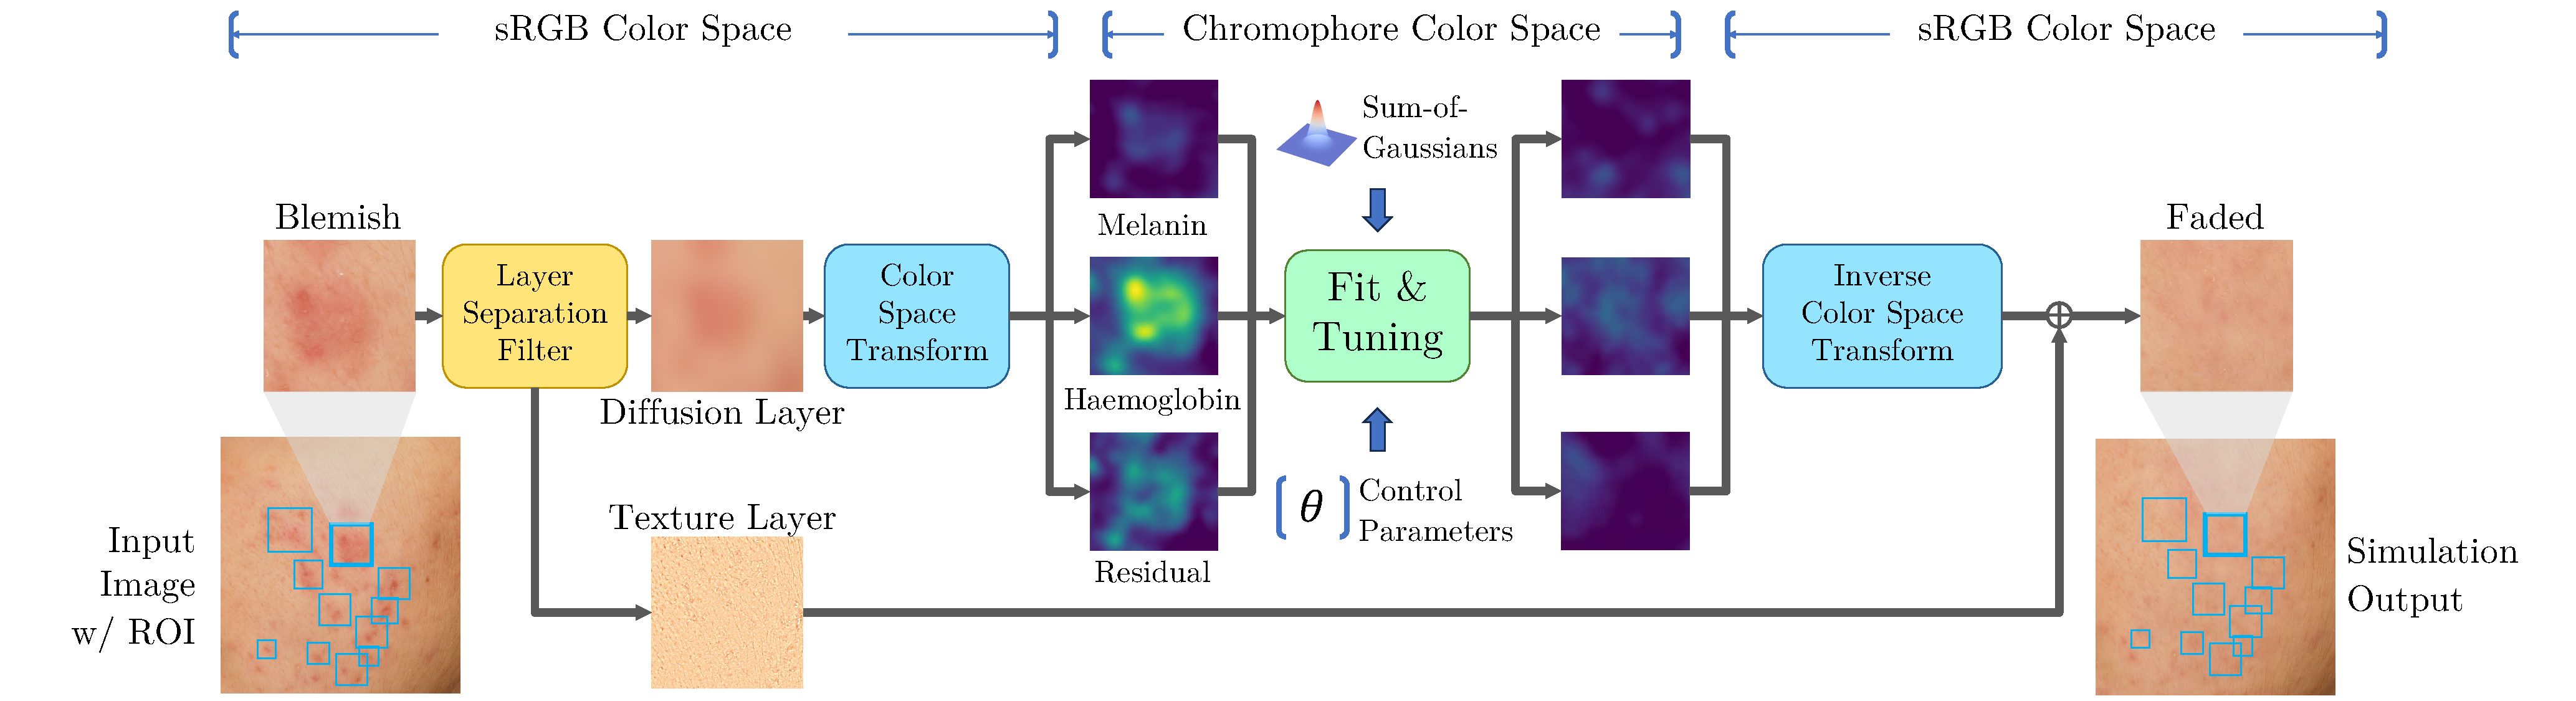
\includegraphics[width=0.94\columnwidth]{Chapter3/system.pdf}
    \caption{An overview of our skin blemish change simulation pipeline. In our pipeline, a box of Region of Interest (ROI) is first used to select the blemish like acne or pigmentation. Then, a \textit{Layer Separation Filter} is applied to separate the texture layer and the diffusion layers. A \textit{Sum-of-Gaussians} model is fitted to each ROI in \textit{Melanin/Heamoglobin} color space, with the parameters of the fitted model adjusted to manipulate the appearance of the blemishes. The modified diffusion layer is summed with the original texture layer to obtain the output.}
    \label{fig:system}
\end{figure}
\subsection{Algorithm Implementations}

As we show in Figure \ref{fig:system}, in our pipeline, we firstly adopted a skin layer separation filter to separate the skin into a surface texture layer (including specular reflections and skin textures) and a scattered chromophore layer. We implemented this by a Gaussian filter with a small variance, small enough to isolate the detail texture of the skin without affecting our assumptions. Then, we converted the image from sRGB to log-RGB space (assume the image is scaled to $[0,1]$ and with no Gamma correction).

We also made a simple GUI for users to draw bonding box or uploading a segmentation map to select desired spots. Then, we fitted for each spot and applied control parameters for each pigmentation channel. After that, the inverse color space transform was applied and the texture layer was bypassed from the input and added to the modified chromophore layer.

In the actual implementation, we performed a number of optimisations to the program. 
\begin{itemize}
    \item First, each channel and each spot can be fitted independently. We then use multi-process parallelism to speed it up.
    \item Second, since $\hat{C_K}$ has explicit partial derivatives, we manually derived its Jacobian matrix. This helped the fitting procedure to quickly compute accurate gradients rather than estimate it numerically.
    \item Third, though we can fit the entire Sum-of-Gaussians model at once, the convergence of the fit will be slow. We thus adopted the following strategy: we gradually put a new $N$-th Gaussian function into the model with $N-1$ functions and fit the updated model, during which the existing parameters are frozen. Finally, we unfreeze all parameters for one more fitting as a fine-tuning. Thus, only one function was fitted each time except for the last one.
\end{itemize}

This algorithm can be represented by the following pseudocode.
\begin{algorithm}
    \caption{Fitting Distribution of a Spot}
    \begin{algorithmic}[1]
    
    \State \textbf{Input:} Spot image patch $X\in\mathbb{R}^3$ from user input
    
    \State \textbf{Preprocessing:}
    % \Indent
        \State $X \gets \gamma^{-1}(X/255.0)$ \Comment{Inverse gamma transformation to linear RGB space}
        \State $X \gets \mathbf{E}^{-1}\cdot\log{X}$ \Comment{Transform to chromophore color space}
    % \EndIndent
    
    \For{each channel $c$ in \{H, M, r\}}
        \State Initialize empty base model $\hat{C_K}(x, y)$
        \For{each Gaussian component $G_i$}
            \State Estimate initial center position $x^{init}_i, y^{init}_i$
            \State Fit $G_i^c(x, y; \mu_x^i, \mu_y^i, \sigma_x^i, \sigma_y^i, \theta, A_i)$
            \State $\hat{C_K} \gets \hat{C_K}+G_i^c$
            \State Freeze parameters of $\hat{C_K}$
        \EndFor
        \State Unfreeze all parameters for final refinement fit
    \EndFor
    
    \State \textbf{Return:} Fitted parameters and fitted color spot image
    
    \end{algorithmic}
    \end{algorithm}

%=== END OF CHAPTER THREE ===
\end{spacing}
\newpage
